\documentclass[fleqn]{beamer}

\usepackage[british]{babel}
\usepackage{verbatim}
\usepackage{graphicx,hyperref,ru,url}

\title[Plaintext Recovery Attacks against SSH]{
Review: Plaintext Recovery Attacks against SSH}

\subtitle{Introduction to Cryptographic Algorithms '12/'13}

\author[Estourgie \& Br\"ucker]{
Raoul Estourgie\\
Ben Br\"ucker}

\institute[Radboud University Nijmegen]{
  Institute for Computing and Information Sciences \\
  Radboud University Nijmegen}

\date[Presentation 5-4-2013]

\begin{document}

  \begin{frame}
    \titlepage
  \end{frame}

  \begin{frame}
    \frametitle{Outline}
    \tableofcontents
  \end{frame}
  
\section{Introduction}

\subsection{What is SSH?}

  \begin{frame}
  \frametitle{What is SSH?}
    \begin{itemize}
      \item Secure Shell (SSH) connects computers securely over insecure network connections.
      \item It was released in 1995 and was designed to replace rlogin, rsh, Telnet and similar insecure protocols. 
      \item The SSH protocol covers authentication, confidentiality and integrity.
      \item Our review article "Plaintext Recovery Attacks against SSH" paper focuses on the OpenSSH implementation.
    \end{itemize}
  \end{frame}
  
\subsection{What is the SSH-BPP protocol?}

  \begin{frame}
  \frametitle{What is the SSH-BPP protocol?}
    \begin{itemize}
      \item The Binary Packet Protocol (BPP) of SSH encrypts a plaintext and then protects it's integrity by appending a MAC value.
      \item Prefixed with 4 byte packet-length, 1 byte padding-length
      \item Suffixed with 4 to 255 bytes of padding
      \item The message is then encrypted with a cypher of choice, for example aes128-cbc.
      \item MAC is calculated over this message and a 32-bit packet sequence number
      \item Mac is appended to the message
    \end{itemize}
  \end{frame}
    
  \begin{frame}
    \frametitle{Schematic of a BPP block}
    \begin{center}
    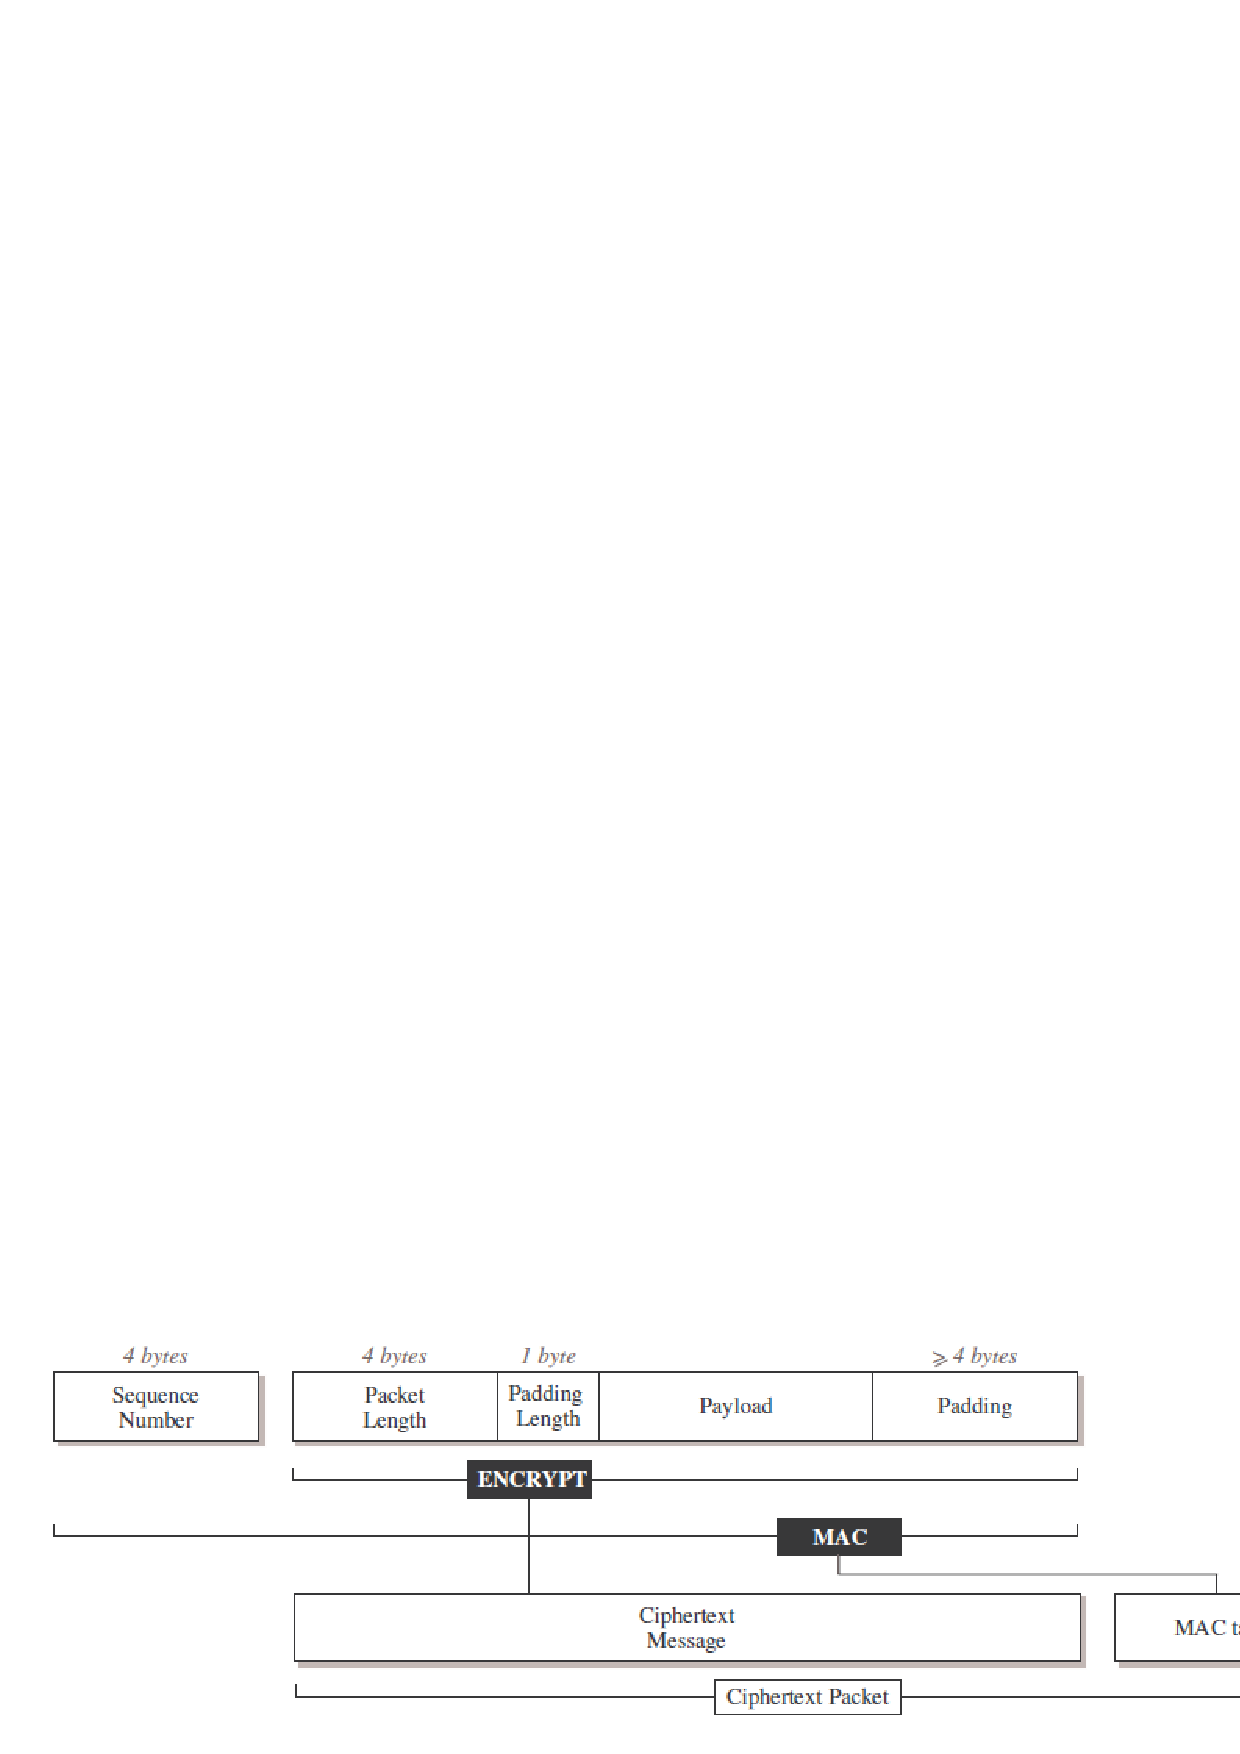
\includegraphics[scale=.4]{SSHBPP.pdf}
    \end{center}
  \end{frame}

  
    \begin{frame}
    \frametitle{Test}
	\begin{itemize}
	\item The packets then form a data stream since the encryption is in CBC mode. 
	\item Every packet $i-1$ on a connection will be the initialization vector (IV) for packet $i$ on the same connection.
	\item For decryption it is essential that the receiver decrypts the first ciphertext block to be able to read the length field.
	\item The SSH protocol also specifies error handling for the BPP protocol. The connection should terminate whenever a transmission error occurs or MAC verification fails. When such a termination happens,the connection should be re-established. Implementations are free to send error messages to their peer when an error occurs.
	\end{itemize}
  \end{frame}
  
  
    \begin{frame}
    \frametitle{Security game}
    \begin{center}
    \includegraphics[scale=.8]{drawing.pdf}
    \end{center}
  \end{frame}
  
\section{Questions}

  \begin{frame}
    \frametitle{Questions}
    \begin{center}
    Questions?
    \end{center}
  \end{frame}
\end{document}
